\chapter{関連する研究と知見}

\section{感情の表現方法}
	感情推定を行う上で,まずは感情の表現方法を定義する必要性がある.
	感情の表現方法の種類として,大きく2種類がある\cite{emotion_analysis_survay}.
	Categorical ModelとDimensional Modelである.

	\subsection{Categorical Model}
		Categorical Modelとは,感情を複数のクラスで表現したものである.
		以下にいくつか例を示す.

		\subsubsection{Ekmanのモデル}
			Ekman\cite{ekman}は怒り,嫌悪,恐れ,喜び,悲しみ,驚きの6つが普遍的な感情であり,生物学的基盤を持つと結論付けている.
			この基準は,異なる文化の人々の表情を読み取ることができるかどうか,である.
			孤立した石器時代の文化で暮らす人々が,他文化の人々の顔の表情を読み取れたかどうかという実験により確認された.

		\subsubsection{Plutchikのモデル}
			Plutchik\cite{plutchik}はEkmanの6感情に加え,信頼と期待を加えた8感情のモデルを提案している.
			本モデルの特徴は喜びと悲しみ,信頼と嫌悪といった形で各感情がそれぞれ対になっている点にある.

		\subsubsection{中村の感情分類}
			中村\cite{kanjou_hyogen_jiten}は,感情表現辞典\cite{kanjou_hyogen_jiten}において,
			言語表現の観点から,感情を「喜, 怒, 哀, 怖, 恥, 好, 厭, 昂, 安, 驚」の10種類に分類している.
			感情表現辞典では,日本の近現代作品の中から様々な感情が入り混じるような微妙な心理を描いた用例を収録している.

	\subsection{Dimensional Model}
		Dimensional Modelとは,感情間の関係を表現するために次元空間を扱うようなモデルのことである.
		感情が連続的であるという仮説の下で表現されたものであり,一般的には2~3次元で表現される.
		主に用いられる次元はvalence(感情価),arousal(覚醒度),dominance(優位性)の3つである.
		valenceは感情が肯定的か否定的かを,arousalは興奮度を,dominanceは感情に対する制御度を示している.\cite{emotion_model_1}\cite{emotion_model_2}
		以下にいくつか例を示す.

		\subsubsection{Plutchikの感情の輪}
			Plutchik\cite{plutchik}は,8つの感情をさらに3段階でレベル分けした,
			2次元の感情モデルを提案している.
			次元はvalenceとarousalの2次元である.
			図\ref{fig:plutchik}は,このモデルを図式化したものである.
			\begin{figure}[H]
				\centering
				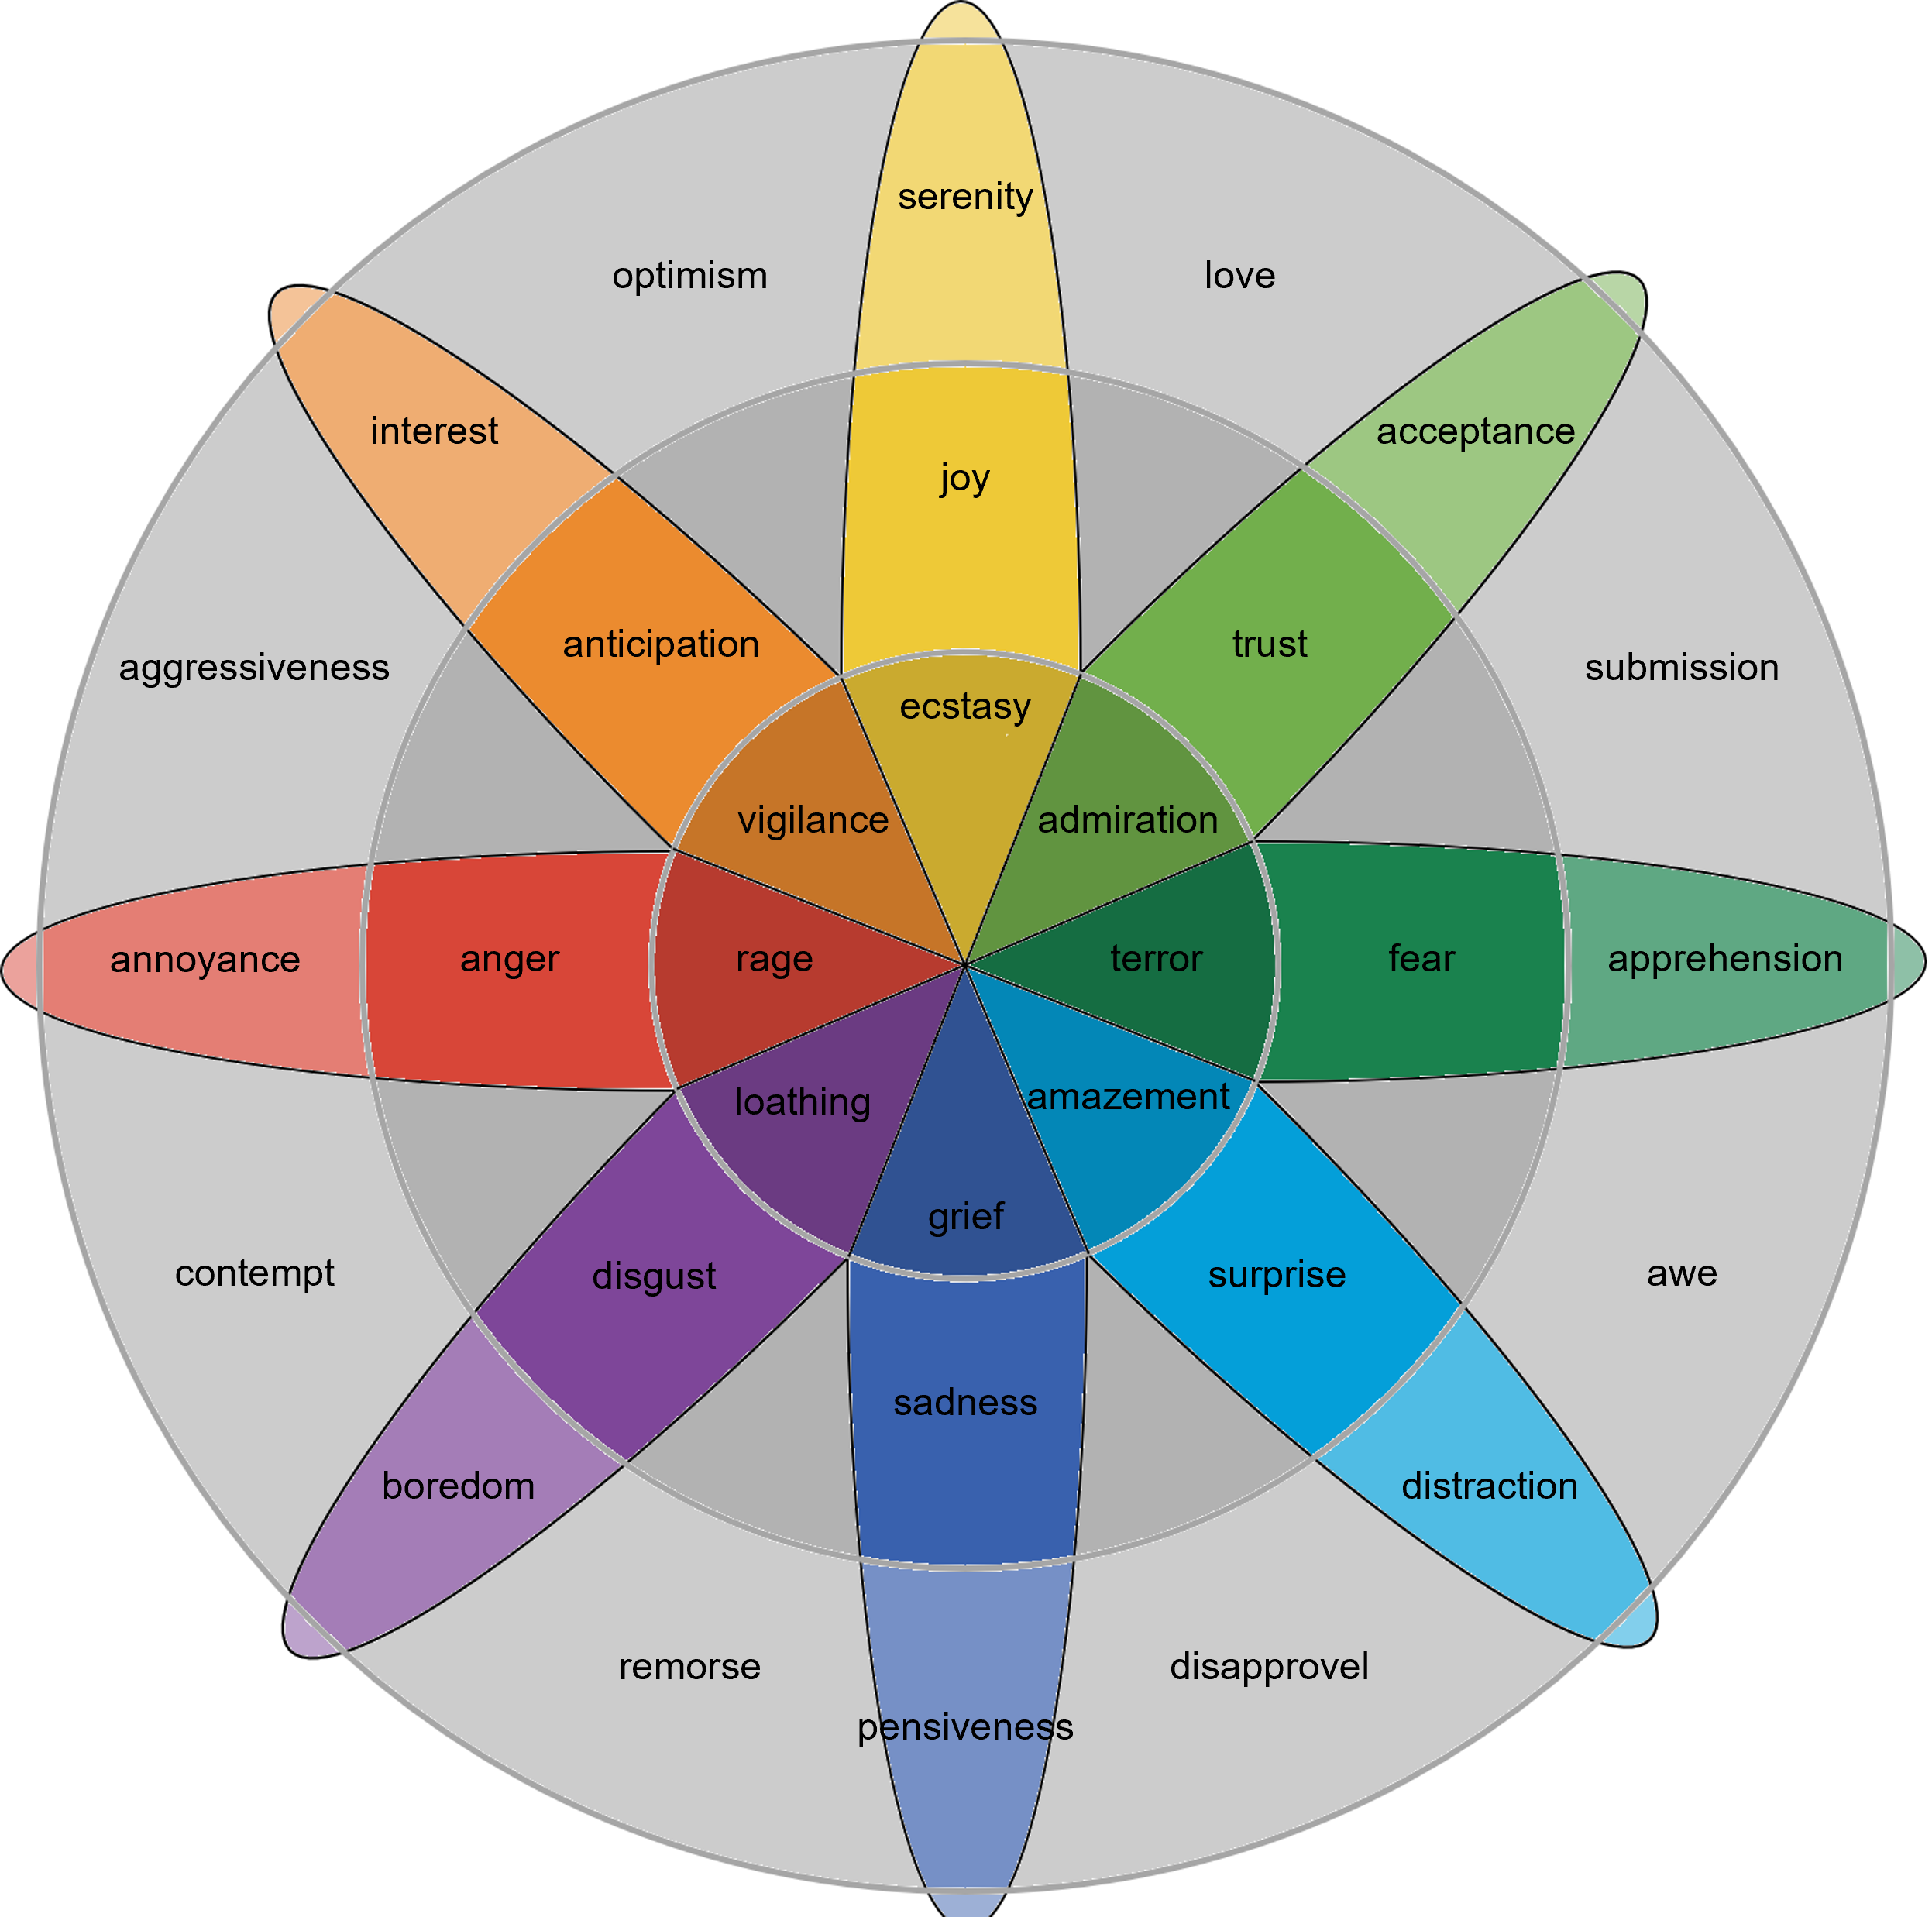
\includegraphics[width=90mm]{./figure/plutchik.png}
				\caption{Plutchikの感情の輪}
				\label{fig:plutchik}
			\end{figure}
			

		\subsubsection{Russellのモデル}
			Russell\cite{russell_2D}は感情をvalence,arousalの2次元で表現する感情モデルを提案した.
			図\ref{fig:russel_2D}は,このモデルを図式化したものである.
			\begin{figure}[H]
				\centering
				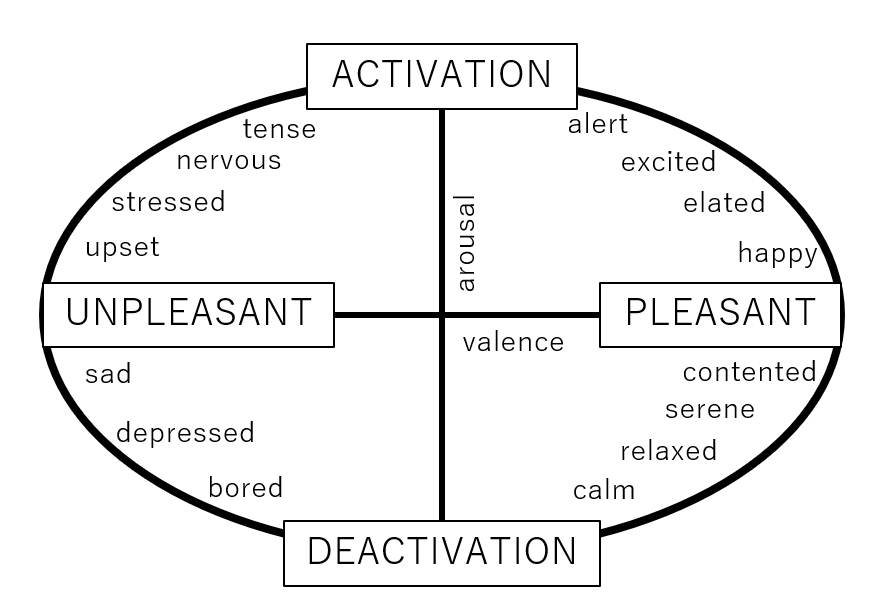
\includegraphics[width=90mm]{./figure/russell.png}
				\caption{Russellのモデル}
				\label{fig:russel_2D}
			\end{figure}

		\subsubsection{Russell, MehrabianのPADモデル}
			RusellとMehrabian\cite{russell_3D}は,Pleasure,Arousal,Dominanceの3次元で表現する感情モデルを提案した.
			PADは各次元の頭文字をとったものである.

\section{コンピュータ上での単語の表現}
	コンピュータは,入力された単語をテキスト情報のまま処理することができない.
	それをかなえるためには,単語のベクトル化が必要となる.

	\subsection{one-hotベクトル}
		one-hotベクトルとは,最も単純な単語のベクトル表現方法である.
		具体的には,語彙内の単語のインデックスに対応した成分だけが1となり,
		その他の成分がすべて0となるようなベクトルである.
		よって,次元数はシステムが扱う語彙数と同数となる.
		図\ref{fig:one-hot-vector}は,サイズが10000語の語彙$V$について,
		語彙内の単語がどのように表現されるのかを表した図である.
		各単語と対応する語彙内のインデックスが括弧内の数字に対応している.
		各ベクトルは,語彙数と同じ10000次元である.
		\begin{figure}[H]
			\centering
			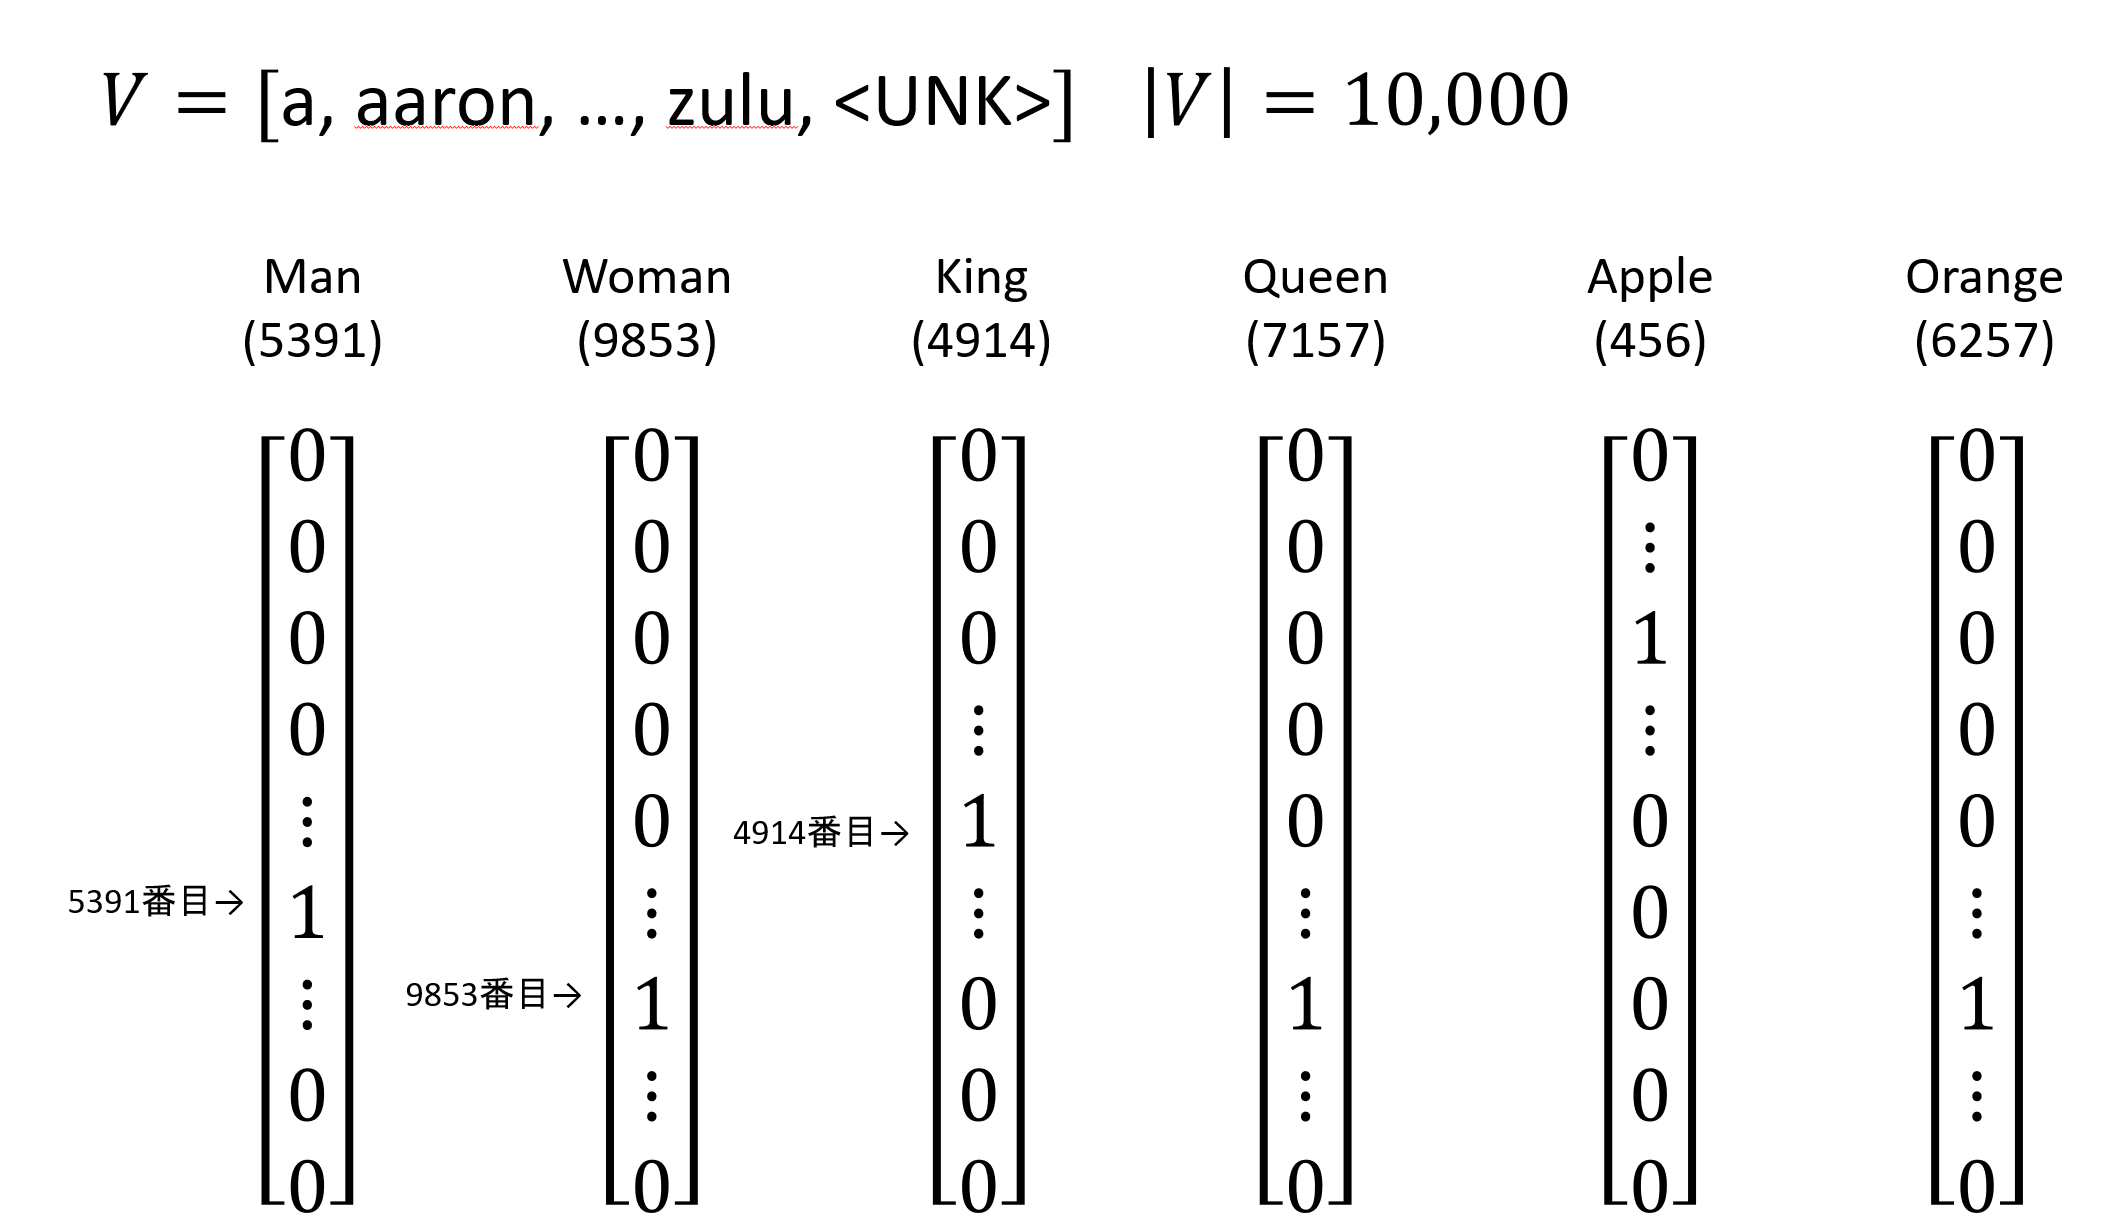
\includegraphics[width=\linewidth]{./figure/one-hot-vector.png}
			\caption{one-hotベクトルの概要}
			\label{fig:one-hot-vector}
		\end{figure}

		one-hotベクトルによる単語ベクトルの表現を行う上でのの問題点として,
		システムの扱う語彙数が増えることにより,単語ベクトルの次元数が同量増えてしまうことが挙げられる.
		また,このような非常に次元の高いベクトルであるにもかかわらず,
		ベクトル内の1成分だけが1で他の成分はすべて0となる.
		よって,単語ベクトルが非常に疎なベクトルとなってしまうため,
		消費するリソースのわりに得られる情報量が少ないということも挙げられる

	\subsection{単語分散表現}
		単語分散表現とは,単語をベクトル空間上の一つの点として捉えるような表現方法のことである.
		単語分散表現は各要素が実数値を持つ,密なベクトルとなっていて,
		システムの語彙数よりも低い次元数のベクトルで表現可能である.
		単語のベクトル同士の計算と単語間の意味関係が対応するのが特徴であり,
		このことからもベクトルの各要素が単語の特徴を表していると考えられている.
		図\ref{fig:word2vec}は,単語分散表現の特徴であるベクトル間の計算と
		意味関係の対応を単純化して示したものである.
		
		\begin{figure}[H]
			\centering
			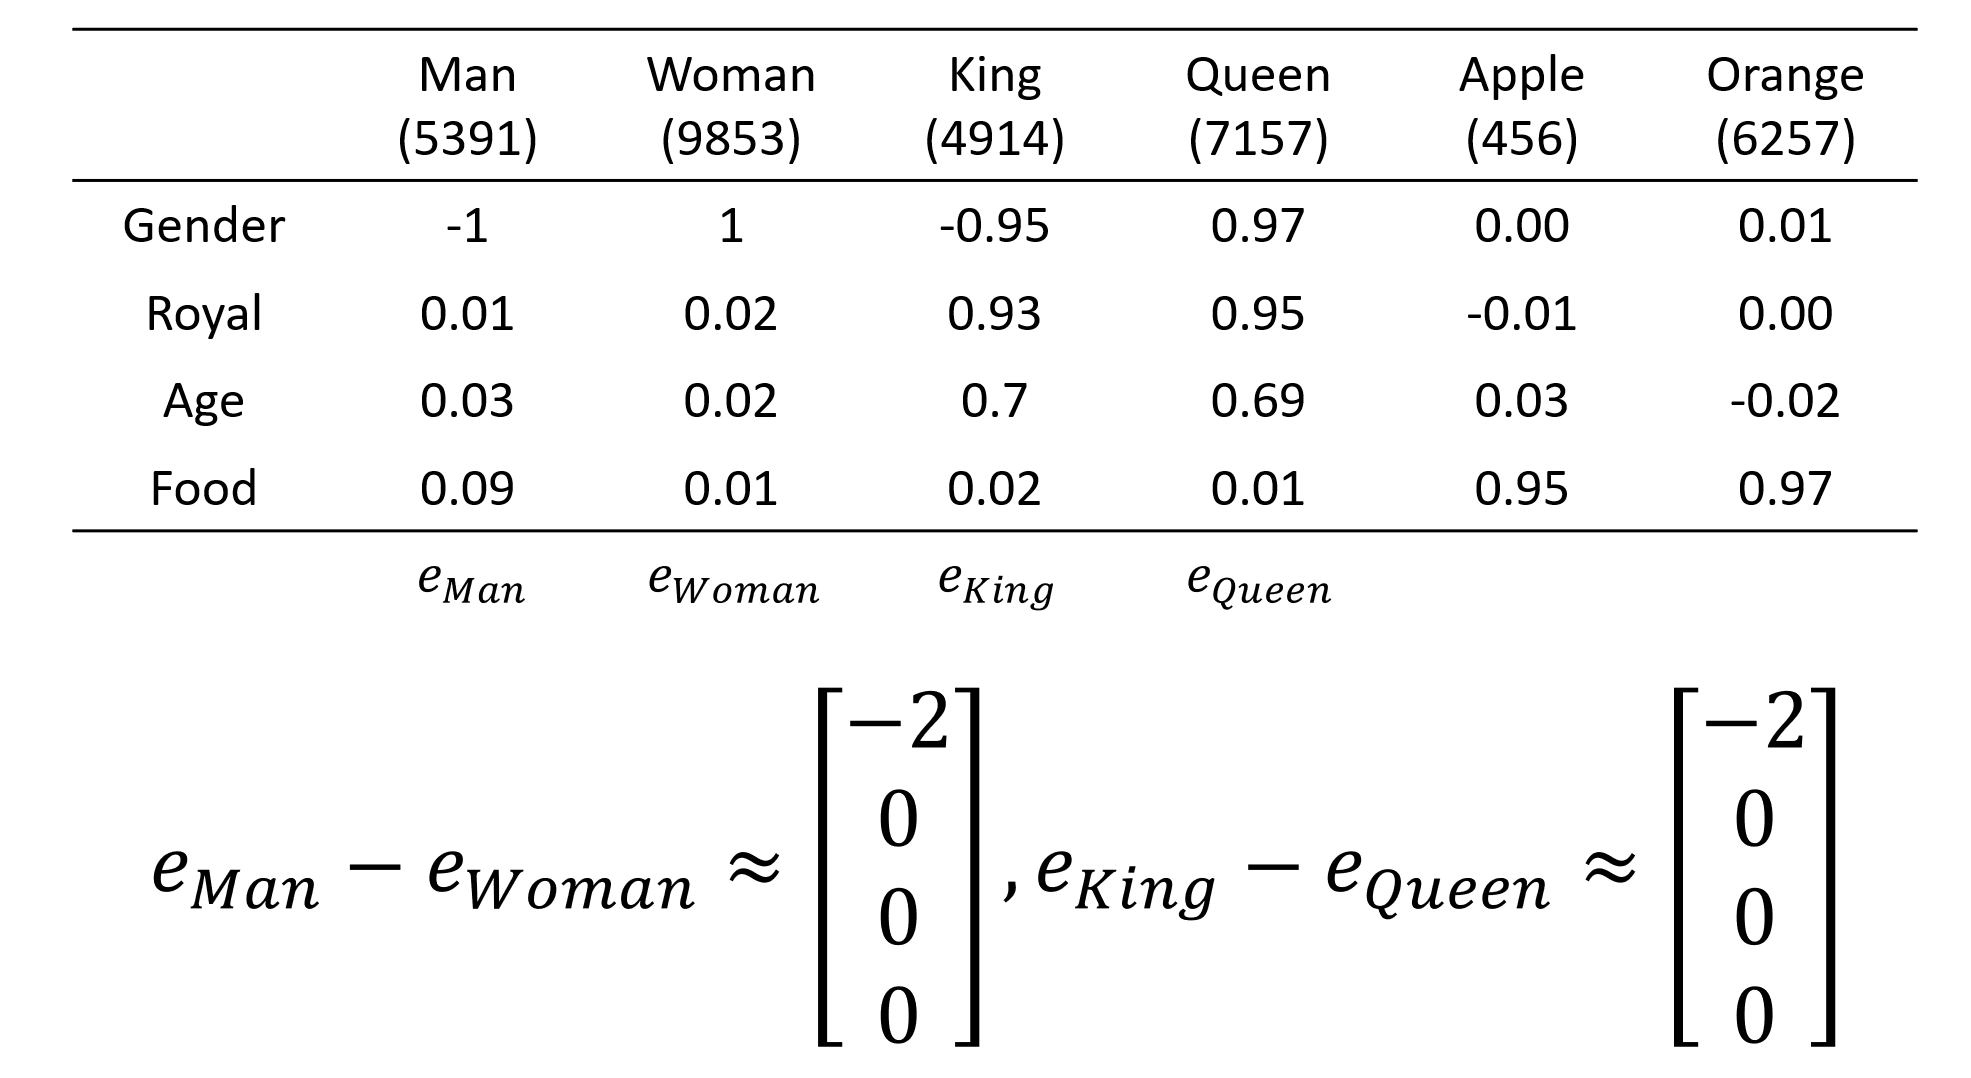
\includegraphics[width=\linewidth]{./figure/word2vec.png}
			\caption{ベクトル同士の計算による単語間の意味関係の取得}
			\label{fig:word2vec}
		\end{figure}

		各成分が特定の意味を持つような4次元のベクトルとして,各単語を表現している.
		この時,"Man"と"Woman"の違いは各ベクトルの差をとることで,
		"Gender"成分にあるということがわかり,
		同様の関係が"King"と"Queen"の間にも認められることがわかる.
		このように,各単語に対応するベクトルの演算結果が,
		単語間の意味関係と対応することになる.
		
		なお,実際に取得される単語分散表現は,より高次元で複雑なものである.
		各成分が持つ意味について人間が把握することは非常に困難であるが,
		ベクトル間の計算と意味関係が一致する性質を踏まえると,
		何かしらの特徴を各成分が表現していると推測される.
		主要な単語分散表現の手法として,Word2Vec\cite{word2vec}やGloVe\cite{glove}などが挙げられる.

\section{CBOWモデルをもとにした単語感情分析手法}
	武内ら\cite{takeuchi}は,Continuous Bag-of-wordsモデルの発想を感情表現の抽出に活用した.

	\subsection{Continuous Bag-of-Wordsモデル}
	Continuous Bag-of-Wordsモデル\cite{word2vec}(以下,CBOWモデルとよぶ)は,Word2Vecを学習するのに用いられる.
	Word2Vecの学習は分布仮説の下で行われる.
	分布仮説とは単語の持つ意味が周囲の単語により決まる,というものである.
	つまり,周りの単語が中心の単語の意味的な要素を持っていることにもなる.

	CBOWモデルは,周りの単語を入力して中央の単語を予測するという形のモデルである.
	図\ref{fig:CBOW}は,CBOWモデルの概要である.

	\begin{figure}[H]
		\centering
		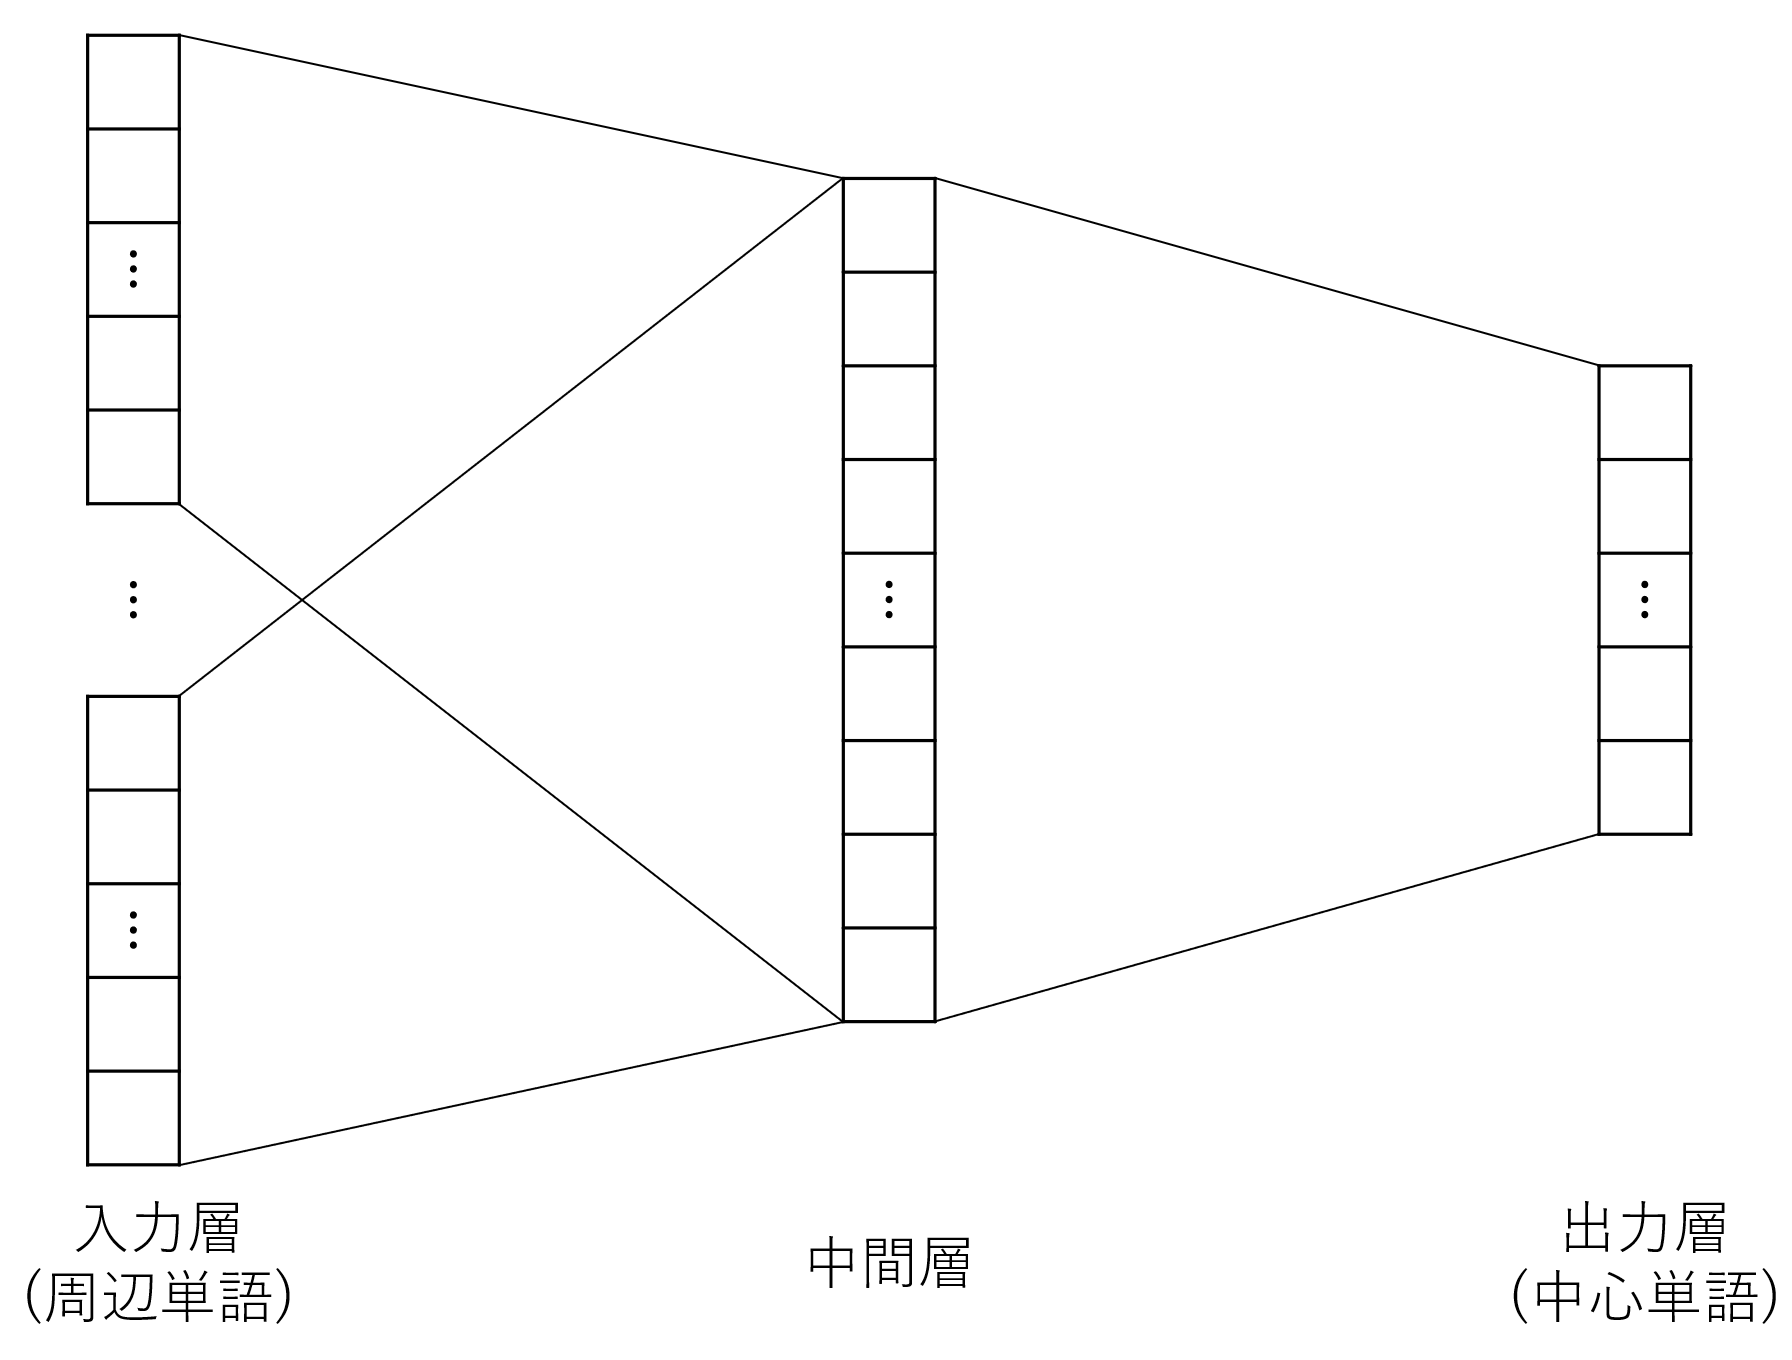
\includegraphics[width=\linewidth]{./figure/CBOW.png}
		\caption{CBOWモデルの概要}
		\label{fig:CBOW}
	\end{figure}

	生成する分散表現の次元数を$d$,語彙数を$V$とすると,
	入力は$V$次元のone-hotベクトル,入力と中間層の間の重みが$(V \times d)$の行列となる.
	中間層は周囲の単語の分散表現の和となり,出力は入力同様に$V$次元のone-hotベクトルで
	中心の単語を出力するという形になる.
	この予測が正しく行えるようにネットワークを学習することで,
	分散表現が単語の意味情報を反映できるようになる.
	

	\subsection{概要}
		\subsubsection{感性語の抽出}
			まず,感情表現辞典\cite{kanjou_hyogen_jiten}から感情と密接にかかわる単語である感性語を取得する.
			この感情表現辞典から得られる感情情報は「喜, 怒, 哀, 怖, 恥, 好, 厭, 昂, 安, 驚」10種類であるため,
			各要素が1つの感情に対応するような10次元のベクトル(以下,感情ベクトルとよぶ)を取得できる.

		\subsubsection{ネットワークの学習}
		テキストデータに対して形態素解析を行い,品詞を絞ったうえで原型に変換する.
		ウィンドウサイズを$W$としたとき,中心の感性語に対し前後$W$個の単語を収集し
		合計$2W+1$個の単語群を一つのデータとする.
		図\ref{fig:takeuchi_dataset}で,周辺単語の収集の様子を示す.
		\begin{figure}[H]
			\centering
			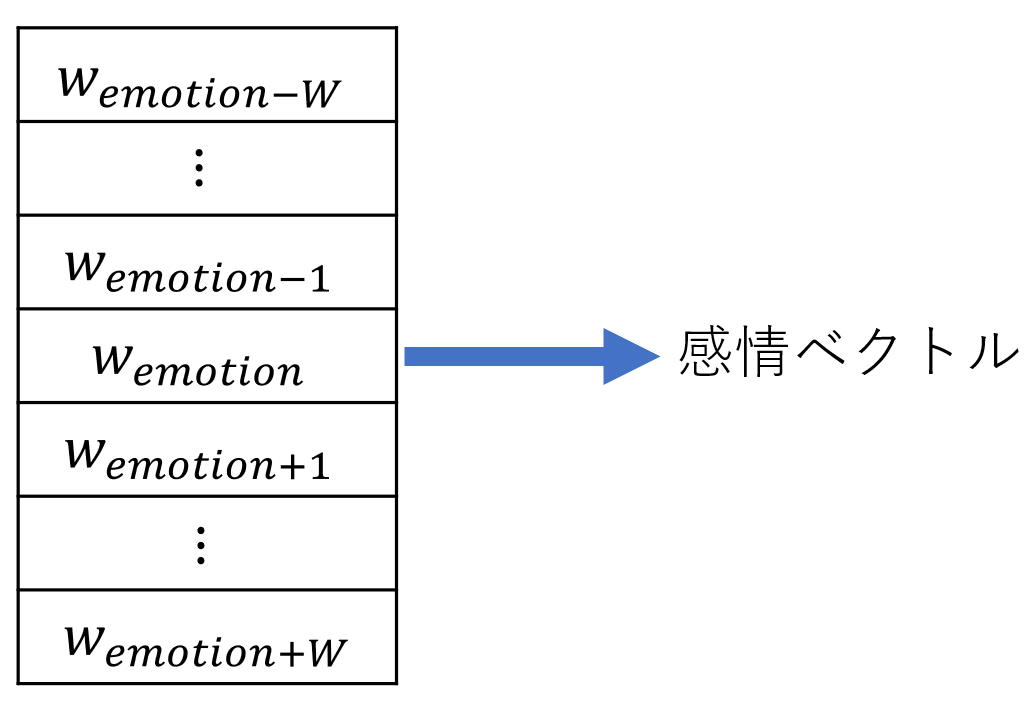
\includegraphics[width=\linewidth]{./figure/takeuchi_dataset.png}
			\caption{データセット生成での単語収集の概要}
			\label{fig:takeuchi_dataset}
		\end{figure}
		入力はそれぞれの単語に対するone-hotベクトルで,
		中間層は感情ベクトルと同じ10次元のベクトルとなる.
		語彙数を$V$としたとき,入力層と中間層の間の重みは,$(V \times 10)$の行列で,
		中間層は入力単語群から変換された10次元のベクトルの和となる.
		この中間層のベクトルをsoftmax層に通したときに,
		中心の感性語が持つ感情ベクトルとの差がなくなるようにしてネットワークを学習する.
		softmax関数は以下の式で示される.
		\begin{equation}
			p_k = \frac{e^{x_k}}{\sum_{i=1}^{10}e^{x_i}}
		\end{equation}
		softmax関数に入力する中間層は10次元で,$x_k$はそのうちの$k$番目の値である.
		softmax関数により,値の総和が1となるような同次元数の出力を得ることができる.
		この時,出力はウィンドウサイズ内の単語を入力した際に推定される感情の確率分布とみなされる.
		以上のような学習により,
		入力層と中間層の間の重みの各行が対応する単語に対する感情ベクトルとなる.

		\subsubsection{出力}
		上述のような学習を行うことにより,各単語に対する10次元の感情ベクトルを取得することができる.
		感情ベクトルの各成分はそれぞれ,「喜, 怒, 哀, 怖, 恥, 好, 厭, 昂, 安, 驚」の感情に対応している.
		これらの感情は,感情表現辞典から得られる情報に対応している.

	\subsection{出力例}
		以下に本手法で得られる出力例を示す.

		\begin{figure}[H]
			\centering
			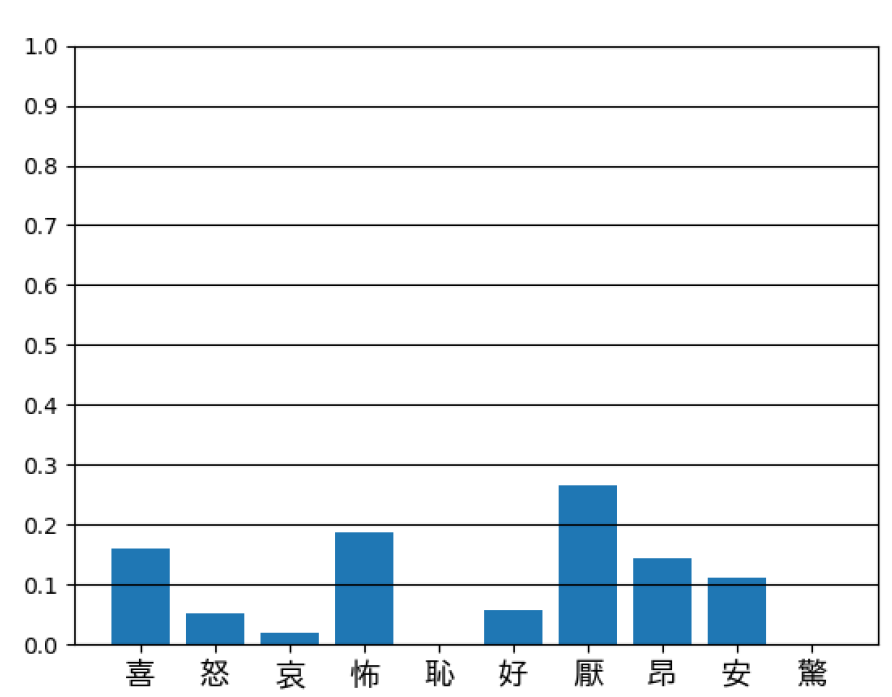
\includegraphics[width=110mm]{./figure/takeuchi_output_toushi.png}
			\caption{本手法で得られる「投資」に対する感情ベクトルの例}
			\label{fig:takeuchi_output_1}
		\end{figure}

		\begin{figure}[H]
			\centering
			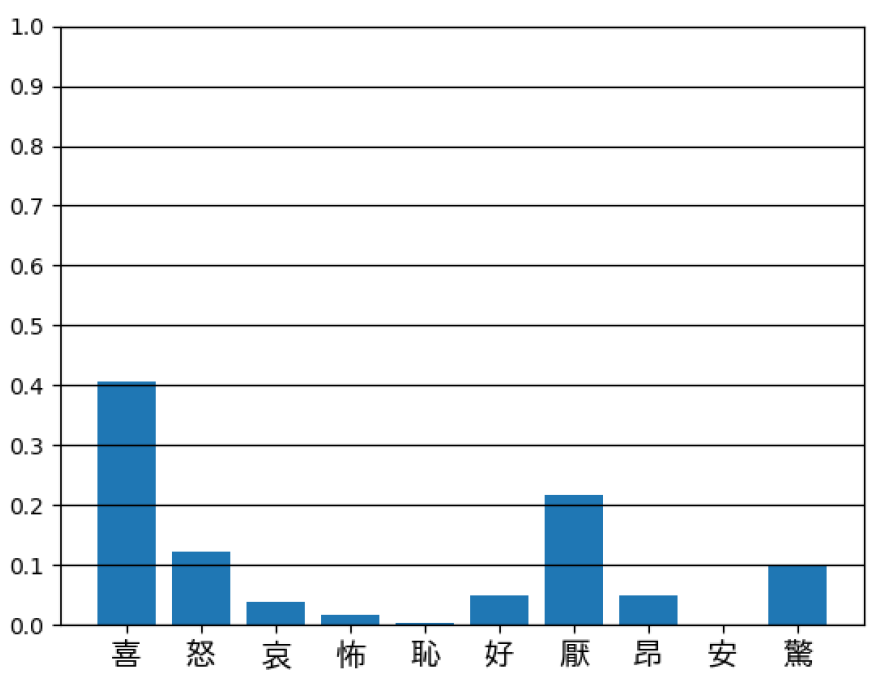
\includegraphics[width=110mm]{./figure/takeuchi_output_seiseki.png}
			\caption{本手法で得られる「成績」に対する感情ベクトルの例}
			\label{fig:takeuchi_output_2}
		\end{figure}

		本手法で得られる感情ベクトルの特徴は,一つの単語に対して,
		想起しうる感情が複数現れることが挙げられる.
		図\ref{fig:takeuchi_output_1}では,「投資」という単語に対する
		感情ベクトルを示している.
		投資に成功して儲けが出た,という文脈においては,
		投資に対してポジティブな印象を持っていると考えられる.
		反面,投資に失敗してしまった,という文脈においては,
		投資に対してあまり良い印象を持っていないと考えられる.
		また,投資をやったことがない,という人にとっては
		怖いものとして扱われるケースも想定される.
		これらの,想定しうる「投資」のイメージを
		感情ベクトルがよく反映しているといえる.
		図\ref{fig:takeuchi_output_2}では,「成績」という単語に対する
		感情ベクトルを示している.
		成績も人や試験等の結果によって抱く印象は様々であり,
		出力でも同様の傾向が見られている.

		このように本手法では,
		単語が用いられる文脈によって想起されうる感情が異なってくることを
		感情ベクトルとして表現することができる.
	
	\vskip\baselineskip
	本研究では,一般単語に対して想起しうる感情情報を抽出している.
	しかし,その情報を使って対話システム等に応用することを考えると,
	単語から想起しうる複数の感情が想起されるのは好ましくない.
	単語がどのような文脈で用いられたかを踏まえたうえでの感情推定ができれば,
	後続のタスクへ適切な感情情報を与えることができる.

\section{BERT}
	Bidirectional Encoder Representations from Transformers\cite{BERT}(以下,BERTとよぶ)は,
	2018年にGoogleから発表された事前学習言語モデルである.
	\subsection{特徴}
		BERTは入力として,文章をトークンに分割したものを用い,出力として,各トークンに対応したベクトルを出力する.
		BERT以前の自然言語処理で主流であったRecurrent Neural Network(以下,RNNとよぶ)ベースのモデルと
		同様の入出力形式である.
		RNNベースのモデルでは,長い文章を入力しても最初の方の情報を保持することができない
		という課題があった.
		しかしBERTでは,Transformer Encoder\cite{attention}により
		トークンの処理に他のトークンの情報を直接的に用いることができる.
		これに伴い,各トークンについてより文脈に即した分散表現を出力することができる.
		図\ref{fig:bert}は,BERTの概要を図式化したものである.
		
		\begin{figure}[H]
			\centering
			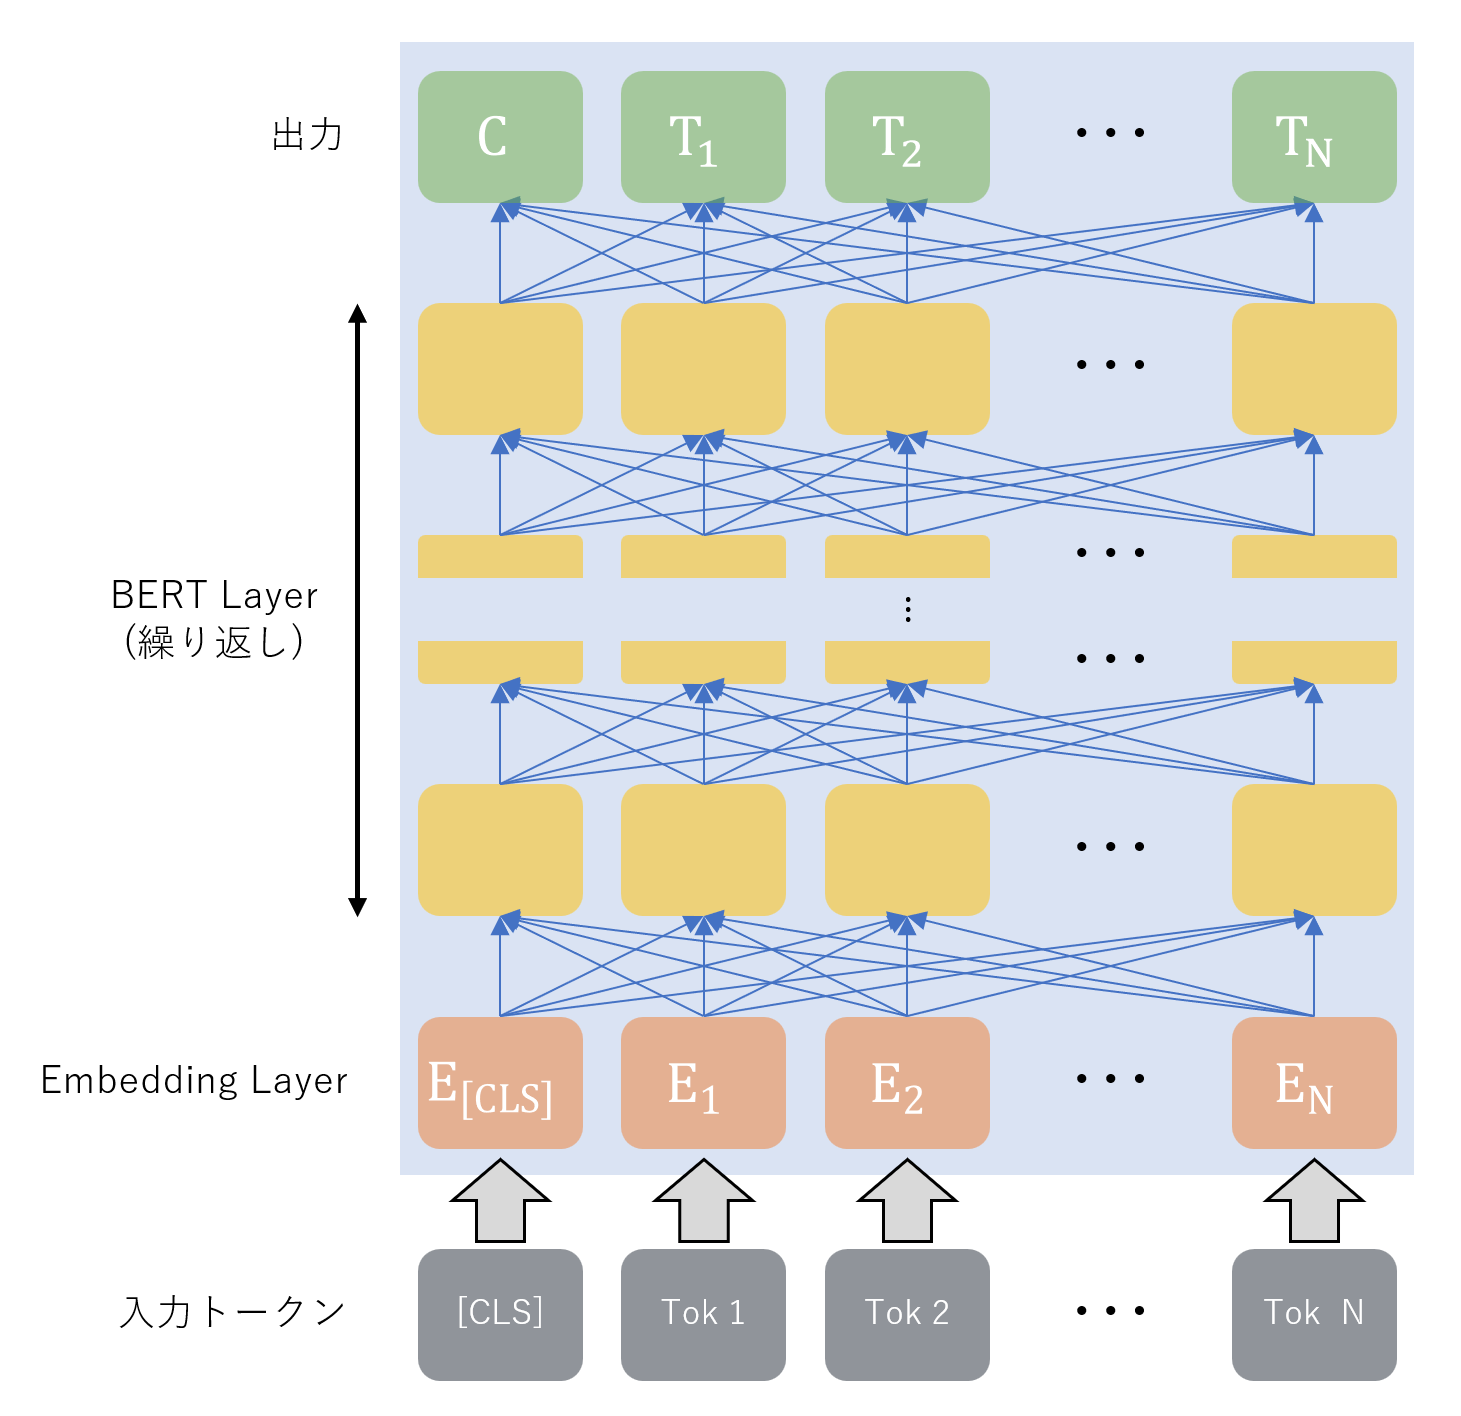
\includegraphics[width=\linewidth]{./figure/bert.png}
			\caption{BERTの概要図}
			\label{fig:bert}
		\end{figure}

	\subsection{BERTから得られる単語分散表現}
		BERTから取得できる単語分散表現の特徴の一つとして,
		同一の単語であっても用いられる文脈によって
		分散表現が変化することが挙げられる.

		例えば,"bank"という単語について考えたとき,
		まったく同じスペルでも文脈に応じて「銀行口座」という意味にも
		「土手」といった意味にもなる.
		Word2Vec等の単語分散表現では,単語に対して分散表現を1対1で対応付けるため,
		こういった多義性を表現することができず,すべて同じ出力となる.
		しかしBERTでは,Traosformer EncoderからなるBert Layerモジュールを繰り返し通すことで
		単語が持つ多義性を分散表現へ反映させることができると考えられている.

		以下,分散表現が多義性を反映していることを確認する簡単な実験\cite{pytorch_advanced}について述べる.
		"bank"という単語を用いた3つの文章を以下に示す.
		\begin{enumerate}
			\item I accessed the bank account.
			\par 日本語訳)銀行口座にアクセスしました.
			\item He transferred the deposit money into the bank account.
			\par 日本語訳)彼は敷金を銀行口座に振り込みました.
			\item We play soccer at the bank of the river.
			\par 日本語訳)土手でサッカーをします.
		\end{enumerate}
		
		文1,文2では"bank"を「銀行口座」という意味で用いているが,
		文3では"bank"を「土手」という意味で用いている.
		入力はEmbedding Layerから得られる"bank"のトークンに
		一対一で対応した分散表現であるが,
		Bert Layerを繰り返し通すことで,
		この分散表現が周囲の単語の影響を受けながら変化していくことになる.
		各文章の"bank"に対応する出力ベクトルの間でコサイン類似度を算出すると
		以下の表\ref{table:bank_compare}のようになる.
		\begin{table}[H]
			\centering
			\caption{各文章の"bank"についての出力ベクトルの類似度比較}
			\label{table:bank_compare}
			\begin{tabular}[H]{c|c}
				\hline
				& cos類似度 \\
				\hline \hline
				文1と文2(同じ意味) & 0.8796 \\
				文1と文3(異なる意味) & 0.4814\\
				\hline
			\end{tabular}
		\end{table}
		% \begin{itemize}
		% 	\item 文1の"bank"と文2の"bank"の類似度 : 0.8796
		% 	\par (どちらも「銀行口座」の意味)
		% 	\item 文1の"bank"と文3の"bank"の類似度 : 0.4814
		% 	\par (文1は「銀行口座」,文3は「土手」の意味)
		% \end{itemize}
		
		このように,"bank"という単語を異なる文章で用いたとしても,
		同じ意味で用いているもの同士であれば,出力ベクトルは類似した出力となる.
		それに対して,"bank"という単語を異なる意味で用いている文章で比較をすると,
		入力としては同じ単語であるにもかかわらず出力ベクトルの類似度は低下する.
		このような結果から,BERTから取得できる単語分散表現には
		文脈考慮性があるということが示唆されている.




